\documentclass{beamer}
\usetheme{CambridgeUS}
\usepackage[utf8]{inputenc}
\usepackage{listings}
\usepackage{tikz}
\usepackage{graphicx}
\usepackage{blkarray}
\usepackage{xcolor}
\usepackage[normalem]{ulem}
\usepackage{verbatim}
\usepackage{amsmath}
\usepackage{arydshln}

% Custom commands
\def\Legendre(#1,#2){%
\begin{pmatrix}
#1\cr
\hdashline[1pt/1pt]
#2\cr
\end{pmatrix}}


\graphicspath{{../res/}}

%Information to be included in the title page:
\title{Alice (and Bob) in Wonderland}
\author{Henk Bierlee}
\institute{Uppsala University}
\date{April 3, 2019}

\definecolor{mygreen}{rgb}{0,0.6,0}
\definecolor{mygray}{rgb}{0.5,0.5,0.5}
\definecolor{mymauve}{rgb}{0.58,0,0.82}

\definecolor{regiongreen}{RGB}{134, 196, 134}
\definecolor{regionpurple}{RGB}{194, 134, 196}
\definecolor{regionorange}{RGB}{255, 150, 0}
\definecolor{regionblue}{RGB}{0, 204, 255}

\lstset{
  backgroundcolor=\color{white},   % choose the background color; you must add \usepackage{color} or \usepackage{xcolor}; should come as last argument
  basicstyle=\footnotesize,        % the size of the fonts that are used for the code
  breakatwhitespace=false,         % sets if automatic breaks should only happen at whitespace
  breaklines=true,                 % sets automatic line breaking
  commentstyle=\color{mygreen},    % comment style
  deletekeywords={...},            % if you want to delete keywords from the given language
  escapeinside={\%*}{*)},          % if you want to add LaTeX within your code
  extendedchars=true,              % lets you use non-ASCII characters; for 8-bits encodings only, does not work with UTF-8
  frame=single,	                   % adds a frame around the code
  columns=flexible,
  keepspaces=true,                 % keeps spaces in text, useful for keeping indentation of code (possibly needs columns=flexible)
  keywordstyle=\color{blue},       % keyword style
  language=C++,                 % the language of the code
  numbers=none,                    % where to put the line-numbers; possible values are (none, left, right)
  rulecolor=\color{black},         % if not set, the frame-color may be changed on line-breaks within not-black text (e.g. comments (green here))
  showspaces=false,                % show spaces everywhere adding particular underscores; it overrides 'showstringspaces'
  showstringspaces=false,          % underline spaces within strings only
  showtabs=false,                  % show tabs within strings adding particular underscores
  stepnumber=2,                    % the step between two line-numbers. If it's 1, each line will be numbered
  stringstyle=\color{mymauve},     % string literal style
  tabsize=2,	                   % sets default tabsize to 2 spaces
  %title=\lstname                   % show the filename of files included with \lstinputlisting; also try caption instead of title
}


\begin{document}

\frame{\titlepage}

\begin{frame}{Problem statement}

\begin{figure}
    \centering
    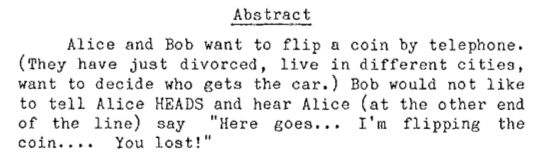
\includegraphics{blum-abstract.png}
    \caption{From \emph{COIN FLIPPING BY TELEPHONE: A PROTOCOL FOR SOLVING IMPOSSIBLE PROBLEMS} by M. Blum (1981)}
    \label{fig:blum-abstract}
\end{figure}

\end{frame}

\begin{frame}{Desired qualities}
    What are some desired qualities in this scenario?
    \begin{itemize}
        \item Fairness
        \begin{itemize}
            \item Both parties have a 50/50 chance of winning
            \item Consequently, neither party can cheat (or it's not in their best interest to attempt to do so)
        \end{itemize}
        \item Non-repudiation: afterwards, either party can prove to a third party who won the game
        \item Cheat-detection: if cheating is attempted, the other party can find out
    \end{itemize}

\end{frame}

\begin{frame}{An (im)practical solution}
    \begin{enumerate}
        \item Alice writes down her call (heads/tails) on paper and locks it in a box
        \item Alice sends the box (but not the key) to Bob
        \item Bob flips a coin and reports the outcome to Alice
        \item Alice reveals who won and sends her key to Bob so he can open the box and verify Alice's claim
    \end{enumerate}
    The box holds Alice's \emph{commitment} to her call. How do we achieve this with classical cryptology methods?
\end{frame}

\part{A classical solution~\cite{blum1981coin}} \frame{\partpage}

\begin{frame}{One-way functions}

    A \emph{normally secure} one-way function~$f$ is an efficiently computable function whose inverse cannot be computed efficiently: given~$f(x)$, it is infeasible to find the input~$x$. \\~\\
    Possible example:~$c = b^e \ (\textrm{mod}\ m)$ (modular exponentiation, solving for~$e$)\\~\\

    A \emph{completely secure} one-way function~$f$ has the additional property that given~$f(x)$, one cannot determine some non-trivial property of~$x$ with~$>50\%$ probability (for instance, the even or oddness of~$x$).
\end{frame}

\begin{frame}{An ideal solution}
    \begin{enumerate}
        \item Alice and Bob agree on a completely secure one-way, one-to-one function~$f$
        \item Alice (randomly) selects an integer~$x$ and computes~$f(x)$
        \item Alice sends only~$f(x)$ to Bob
        \item Bob (randomly) guesses whether~$x$ is even or odd
        \item Alice reveals whether Bob was correct (and sends the original input~$x$ so Bob can verify that~$f(x) = x$)
    \end{enumerate}

    $f(x)$ constitutes Alice's \emph{commitment} to her call of $x$. Since $f$ is one-to-one, there is no other value that $f$ maps to $f(x)$.
\end{frame}


\begin{frame}{Another approach}
    However, completely secure one-way functions are hard to find and may not exist at all! But maybe we can do it with a normally secure one-way function?\\~\\

    A \emph{two-to-one} function~$f$ maps exactly two elements from its domain to each element of its range: for each input~$x$, there always exists a second value~$y \neq x$ for which~$f(y) = f(x)$.\\~\\

    Example: \only<1>{$f(x) = |x|$?}
    \only<2>{$f(x) = \frac{1}{|x|}$}

\end{frame}

\begin{frame}{A classical solution}{Basic concept}

    Consider a normally secure one-way, two-to-one function $f$ with two additional properties:
    \begin{itemize}
        \item Given~$x$, it's hard to find~$y \neq x$, such that~$f(y) = f(x)$
        \item The elements of an input pair~$x, y$ can be distinguished from each other
        \begin{itemize}
            \item Example: when~$x$ is even,~$y$ is odd
        \end{itemize}
    \end{itemize}

    \pause
    Then, basically as before: Alice randomly selects~$x$, sends~$f(x)$ to Bob, Bob guesses the property, and Alice sends~$x$ for verification\\~\\

    Alice's inability to find a second, distinct value~$y$ that~$f$ will also map to~$f(x)$ prevents her from cheating.
\end{frame}

\begin{frame}{A classical solution}
    \begin{enumerate}
        \item We can efficiently compute an integer~$n=p_{1}*p_{2}$, where
        \begin{itemize}
            \item $p1, p2$ are two random, large (80-digit) primes
            \item $p_1 \equiv p_2 \equiv 3\ (\textrm{mod}\ 4)$
            % \item Given $n$, we cannot be efficiently compute $p_1$ and $p_2$ (since prime factorisation is computationally hard)
        \end{itemize}
        \item The Jacobi~\footnote{Generalisation of the Legendre symbol} symbol~$\Legendre(x,n)$ (for odd positive integers~$n$ and arbitrary integers~$x$) has values~$0$,~$+1$ or~$-1$ and is efficiently computable
        \item The group $\mathbb{Z}_n^*$ holds all integers less than $n$ which are relatively prime to $n$ (meaning that numbers in $\mathbb{Z}_n^*$ have no common divisors with~$n$ except~$1$)
    \end{enumerate}

    \pause
    Roughly speaking, $n$ (from point 2) can provide a one-way  function $f_n$ with inputs from~$\mathbb{Z}_n^*$ of which exactly half the solutions of the inverse will have~$\Legendre(x,n)=+1$ (and the other half~$\Legendre(x,n)=-1$).
\end{frame}

% \begin{frame}{A classical solution}{Central theorem}
%     Putting this all together it turns out that: For $a \in \mathbb{Z}_n^*$, exactly half the solutions of $a \equiv x^2 \ (\textrm{mod}\ 4)$ have $\Legendre(x,n) = +1$ (the other half have $\Legendre(x,n) = -1$) (uniformity)

%     In other words, we can use $n$ as a coin-flip generator, because $\mathbb{Z}_n^*$ contains numbers


%     For some $x,y \in \mathbb{Z}_n^*$, half the solutions of the equitaion $y^2 \equiv x^2 \ (\textrm{mod}\ 4)$
%     For any odd positive integer $n$, the following statements are equivalent:

%     \begin{enumerate}
%         \item There exist $x,y \in \mathbb{Z}_n^*$ such that $x^2 \equiv y^2 \ (\textrm{mod}\ 4)$ and $\Legendre(x,n) \not = \Legendre(y,n)$ (two-to-one + distinguishing property)
%         \item For $a \in \mathbb{Z}_n^*$, exactly half the solutions of $a = x^2 \ (\textrm{mod}\ 4)$ have $\Legendre(x,n) = +1$ (the other half have $\Legendre(x,n) = -1$) (uniformity)
%     \end{enumerate}

%     If have $n$
%     which is the product of primes (like point 2)
%     Jacobi symbol~$f_n(x) = \Legendre(x,n)$ is a normally secure two-to-one function for $n$ (from point 2) and for any $x$ in the group $\mathbb{Z}_n^*$
% \end{frame}

% \begin{frame}{A classical solution}{Central theorem}
%     It turns out that if we have
%     For any odd positive integer $n$, the following statements are equivalent:

%     \begin{enumerate}
%         \item There exist $x,y \in \mathbb{Z}_n^*$ such that $x^2 \equiv y^2 \ (\textrm{mod}\ 4)$ and $\Legendre(x,n) \not = \Legendre(y,n)$ (two-to-one + distinguishing property)
%         \item For $a \in \mathbb{Z}_n^*$, exactly half the solutions of $a = x^2 \ (\textrm{mod}\ 4)$ have $\Legendre(x,n) = +1$ (the other half have $\Legendre(x,n) = -1$) (uniformity)
%     \end{enumerate}

%     If have $n$
%     which is the product of primes (like point 2)
%     Jacobi symbol~$f_n(x) = \Legendre(x,n)$ is a normally secure two-to-one function for $n$ (from point 2) and for any $x$ in the group $\mathbb{Z}_n^*$
% \end{frame}


\begin{frame}{A classical solution}{Pros and cons}
    \begin{itemize}
        \item[$+$] Non-repudiation: if all messages are signed, then the outcome of the protocol can be proven to an outside source (ie. a judge)
        \item[$+$] Cheat-detection: one party (or a trusted third party) constructs $n$, which can be tested for the desired properties
        \item [$-$] The security of the algorithm depends on the prime factors of~$n$ being secret
        \begin{itemize}
            \item In other words, the assumption that prime factorisation is \emph{computationally hard}
            \item But advances in algorithm design makes this an unsure assumption
            \item For example, Shor's algorithm can factorise primes efficiently on quantum hardware~\cite{bernstein2017post}
        \end{itemize}
    \end{itemize}
\end{frame}


% \begin{frame}{Presentation overview}

% \emph{Quantum cryptography:
% Public key distribution and coin tossing}\\
% \quad by Charles H. Bennett and G. Brassard (1984)
% \vfill

% \begin{itemize}
%     \item \sout{Problem statement}
%     \vfill
%     \item Recap: behaviour of polarised photons
%     \vfill
%     \item Remote quantum coin-toss protocol
%     \vfill
%     \item Drawbacks
%     \vfill
%     \item Questions
%     \vfill
% \end{itemize}
% \vfill

% \end{frame}
\part{A quantum solution~\cite{bennett2014quantum}} \frame{\partpage}

\begin{frame}{Behaviour of polarised photons}{Encoding bits as photons}

    \begin{itemize}
        \item Light exists of photon particles which can be polarised at any angle with a polarising filter (up, right, diagonal, ..)
        \item This means we can encode a bit of information~(0/1) into a photon in multiple ways, or \emph{bases} (rectilinear basis, diagonal basis, ..)
        \item A photon's polarisation can be measured with a filter, but..
        \begin{itemize}
            \item Rectilinear photon + rectilinear filter = deterministic outcome
            \item Rectilinear photon + diagonal filter = random outcome
        \end{itemize}
        \item Since a photon cannot be duplicated (`no-cloning theorem') and it loses its original polarisation after measurement, you only get one chance to measure it.
    \end{itemize}

% Light exists of individual photon particles, which can be polarised at any angle using polarising filters.
% Four of these polarisation axis are important to us: two rectilinear (0 degrees, 90 degrees) and two diagonal (45 degrees, 135 degrees).
% To measure the orientation of a polarised photon, one can again use polarising filters.
% If the orientation (or basis) of the filter matches the orientation of the photon, the photon will pass through, and if the filter is orthogonal to the photon, the photon will not pass through.
% In other words, rectilinear photons can be measured accurately 100\% of the time (deterministically) if one uses the `correct', rectilinear filter, since the difference in angle between photon and a filter at 0 degrees is always either 0 or 90 degrees.

% But suppose the difference is 45 degrees, such as is always the case when you try to measure rectilinear photons with a `wrong', diagonal filter.
% It happens that the probability of photons passing through this filter is exactly 50\%, so the measurement will tell you exactly nothing about the original polarisation.
% Photons that did pass through now have the same polarisation as the filter, so re-measuring them tells you nothing about their original orientation.
% Furthermore, we cannot simply clone photons and perform multiple measurements.
% Essentially, you only get one chance to measure a photon, and even though there is theoretically infinite information in a photon (if the polarisation is on a continuous spectrum), measurement will only yield one bit of information.

\end{frame}

\begin{frame}{Behaviour of polarised photons}{Example}
\begin{figure}
    \centering
    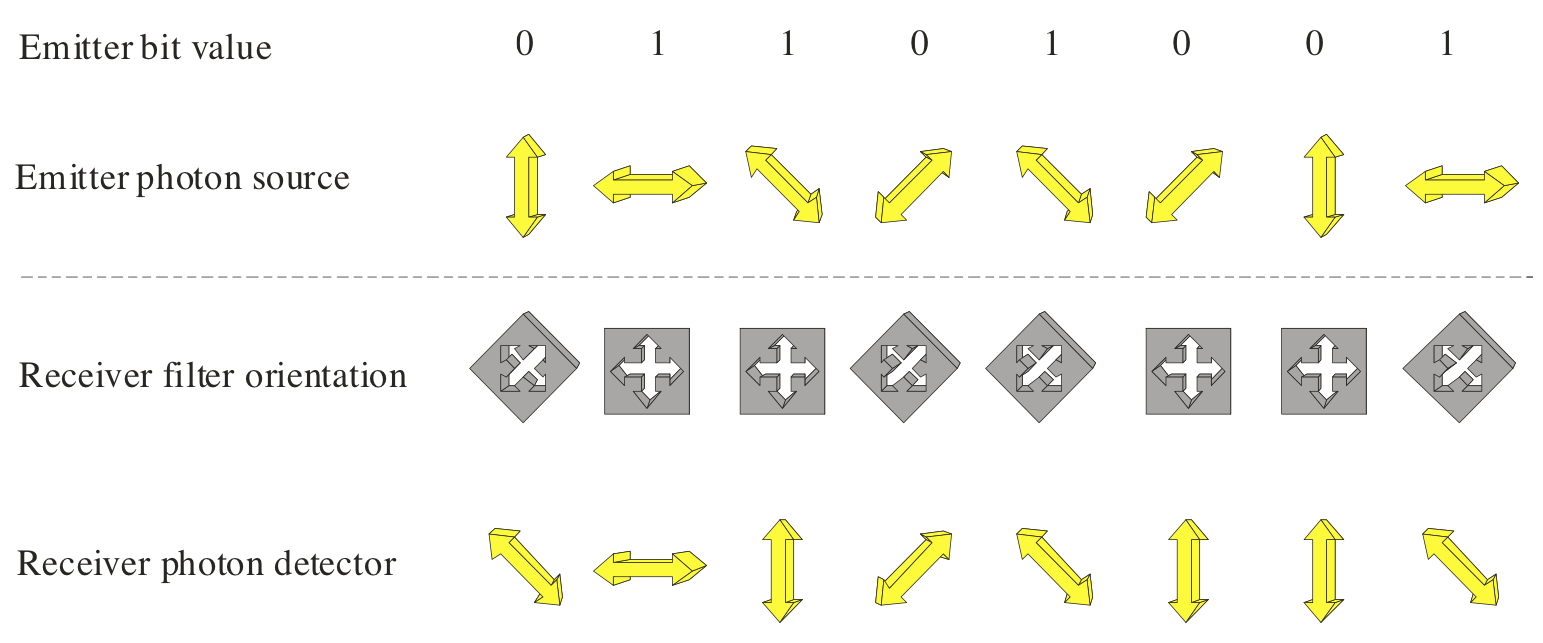
\includegraphics[width=\textwidth, keepaspectratio]{photon-behaviour}
    \caption{From the Cryptology lecture slides (Feb. 27, 2019)
    % When a photon is measured in the way it was polarised, we will know its original orientation (and the original bit value). If it is measured with the other filter, we get a random bit value.
    }
    \label{fig:photon_behaviour}
\end{figure}


\end{frame}

\begin{frame}{A quantum solution}

\begin{figure}
    \centering
    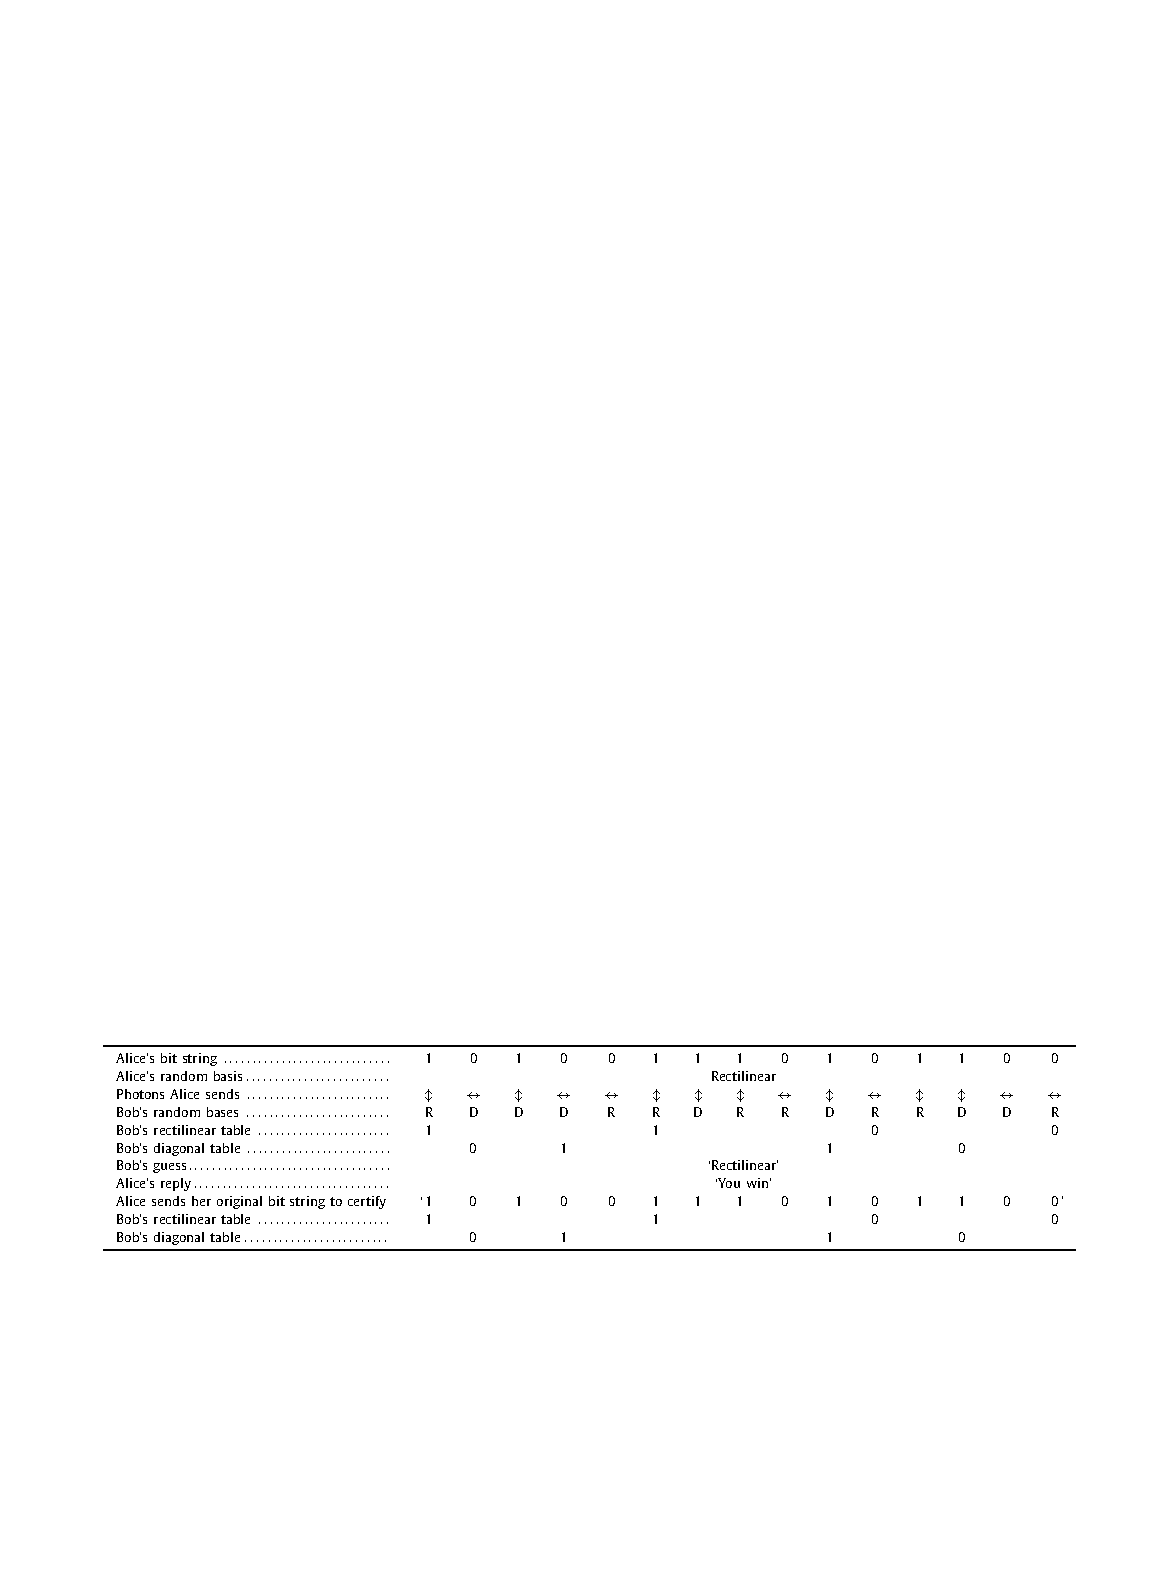
\includegraphics[width=\textwidth, keepaspectratio]{coin-table.pdf}
    \caption{Table from \emph{Quantum cryptography: Public key distribution and coin tossing}}
    \label{fig:coin_table}
\end{figure}

\only<1>{1. Alice encodes a random bit-string with a randomly chosen basis and sends them to Bob}
\only<2>{2. Bob randomly chooses a basis for each photon and fills corresponding measurement table and makes a guess}
\only<3>{3. Alice reveals the correct basis and sends original bit-string over classic communication channel}
\only<4>{4. Bob verifies that Alice didn't cheat by comparing bit-string to corresponding measurement table}
\end{frame}


\begin{frame}[plain,c]
    \begin{center}
        \Huge More volunteers..?
    \end{center}
\end{frame}

\begin{frame}{A quantum solution}{Practical application}
\begin{itemize}
    \item We need \emph{good} quantum hardware..
        \begin{itemize}
            \item Otherwise Alice might accidentally send multiple photons, allowing Bob to measure multiple times and guess the filter with $>50\%$ probability
        \end{itemize}
    \item ..but we don't want \emph{perfect} quantum hardware.
        \begin{itemize}
            \item Otherwise Alice could cheat by `entangling' photons with the so-called Einstein-Podolsky-Rosen effect
            \item In practice likely impossible to achieve
        \end{itemize}
\end{itemize}
First experimental quantum coin-toss already performed at the Laboratory for Communication and Processing of Information (LTCI) in Paris!
\end{frame}

\begin{frame}{A quantum solution}{Pros and cons}
    \begin{itemize}
        \item[+] By the properties of quantum mechanics, it is impossible to cheat:
        \begin{itemize}
            \item Alice cannot cheat, because she can predict only one table with 100\% accuracy, but not the other
            \item Bob cannot cheat, because the photons give no information as to the basis he has to guess
        \end{itemize}
        \item[-] No non-repudiation: quantum cryptography does not provide digital signatures
    \end{itemize}

    So we rely on the \emph{laws of physics} instead of on \emph{computational complexity}
\end{frame}

\begin{frame}[plain,c]
%\frametitle{A first slide}

\begin{center}
    \Huge \emph{Questions..?}
\end{center}

\end{frame}


\begin{frame}[plain,c]
%\frametitle{A first slide}

\begin{center}
    \Huge \emph{Thank you for listening!}

\end{center}
\vfill
    \large
    Report, slides and demo source code available at:\\ \quad \url{https://github.com/hbierlee/quantum-coin-toss}

\end{frame}

\begin{frame}{References}
        % \frametitle{References}
        \bibliographystyle{amsalpha}
        \bibliography{tex/sources}
\end{frame}

\end{document}


    % \begin{itemize}
    %     \item \begin{verbatim}
    %          0 1 0 1 0 0
    %         \end{verbatim}
    %     % \item \begin{verbatim}
    %     %         RECTILINEAR
    %     %     \end{verbatim}
    % \end{itemize}
